\hypertarget{meta-analysis}{\subsection{Meta-analysis}} 
\label{sec:meta-analysis}
To summarize, we evaluate \nummodels language models (\eg \gptdavinci, \bloom) on \numcorescenarios \core scenarios (\eg \naturalquestions, \imdb) for \nummetriccategories metric categories (\eg accuracy, fairness).
Here, we use our comprehensive evaluation to provide answers to important questions in the field like whether model accuracy correlates with scale or if more robust models are less biased.

\begin{figure*}
\centering
  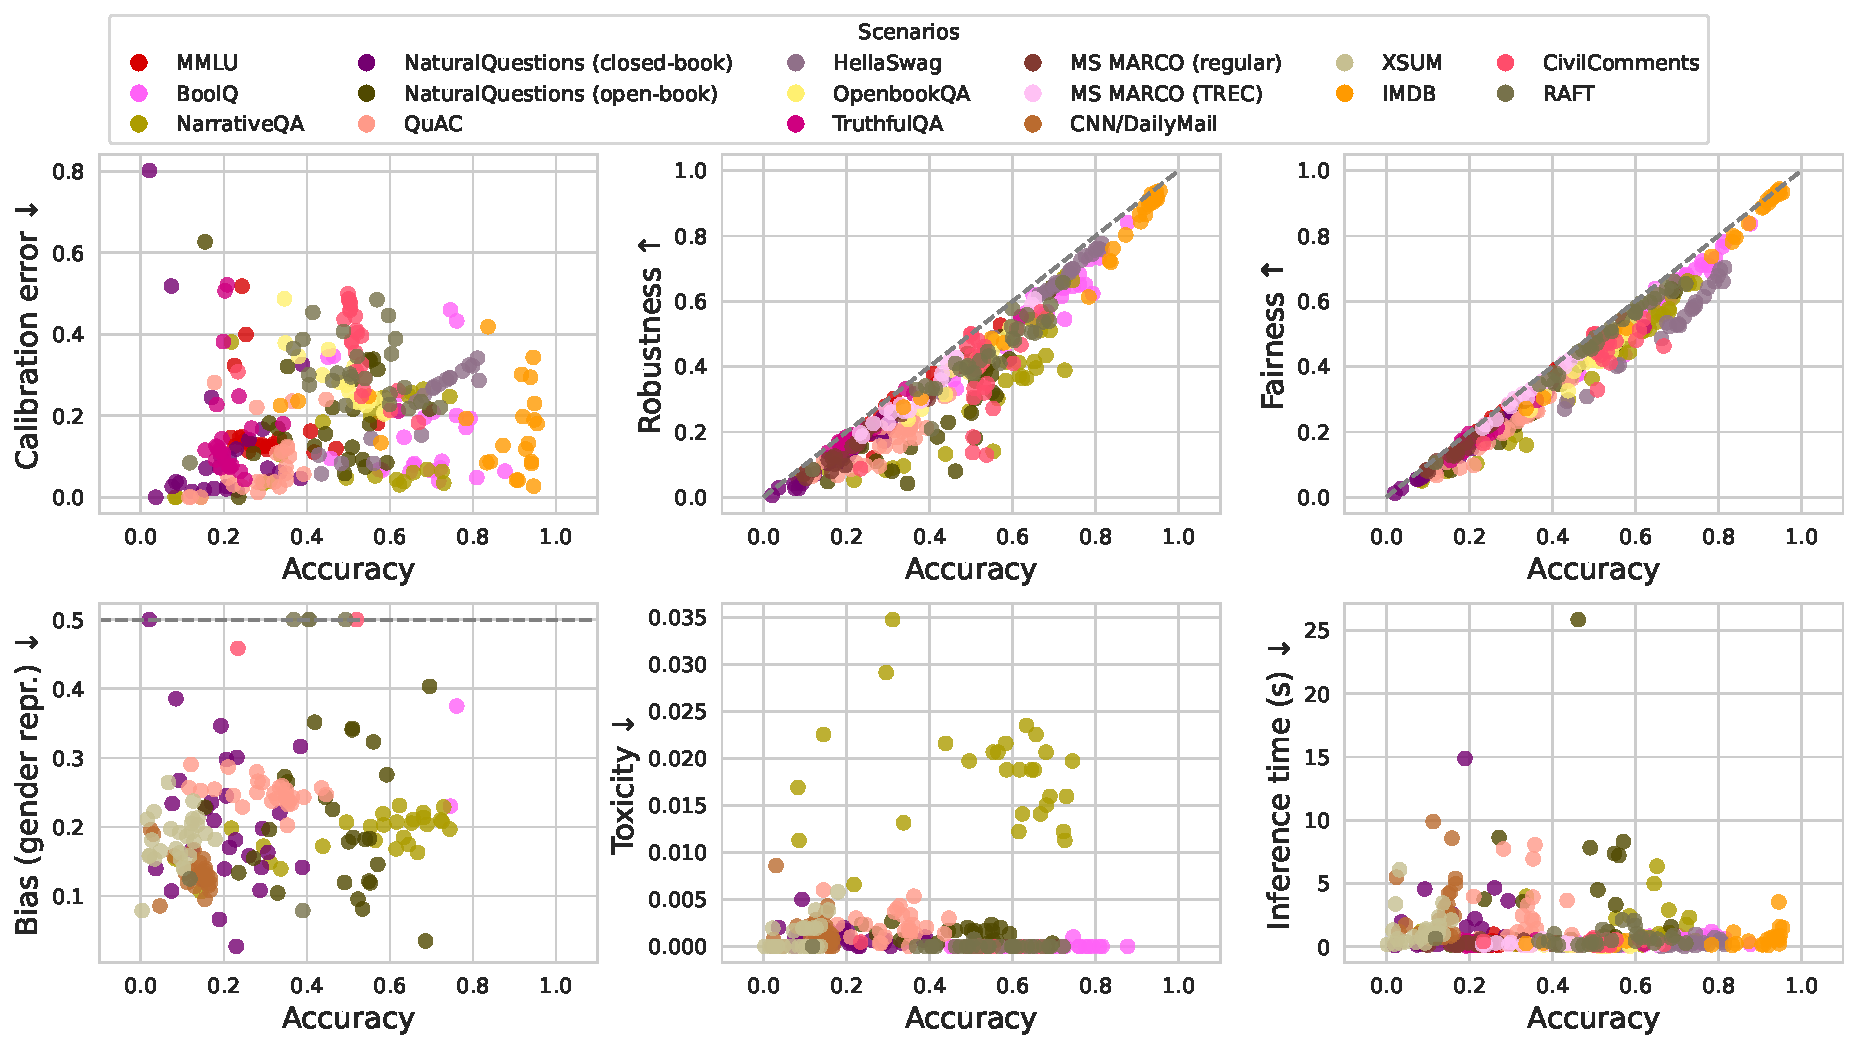
\includegraphics[width=\textwidth]{plots/accuracy_v_x.pdf}
  \caption{\textbf{Accuracy vs. X.} The relationship between accuracy (x-axis) and each of the \numnonaccuracymetriccategories metrics (calibration, robustness, fairness, social bias, toxicity, efficiency) we study in this work across all \core scenarios and for all models.
  For calibration error, we measure ECE-10; for bias, we measure bias in gender representation; and for efficiency, we measure denoised inference time. 
  }
  \label{fig:acc-X}
\end{figure*}

\begin{figure*}
\centering
  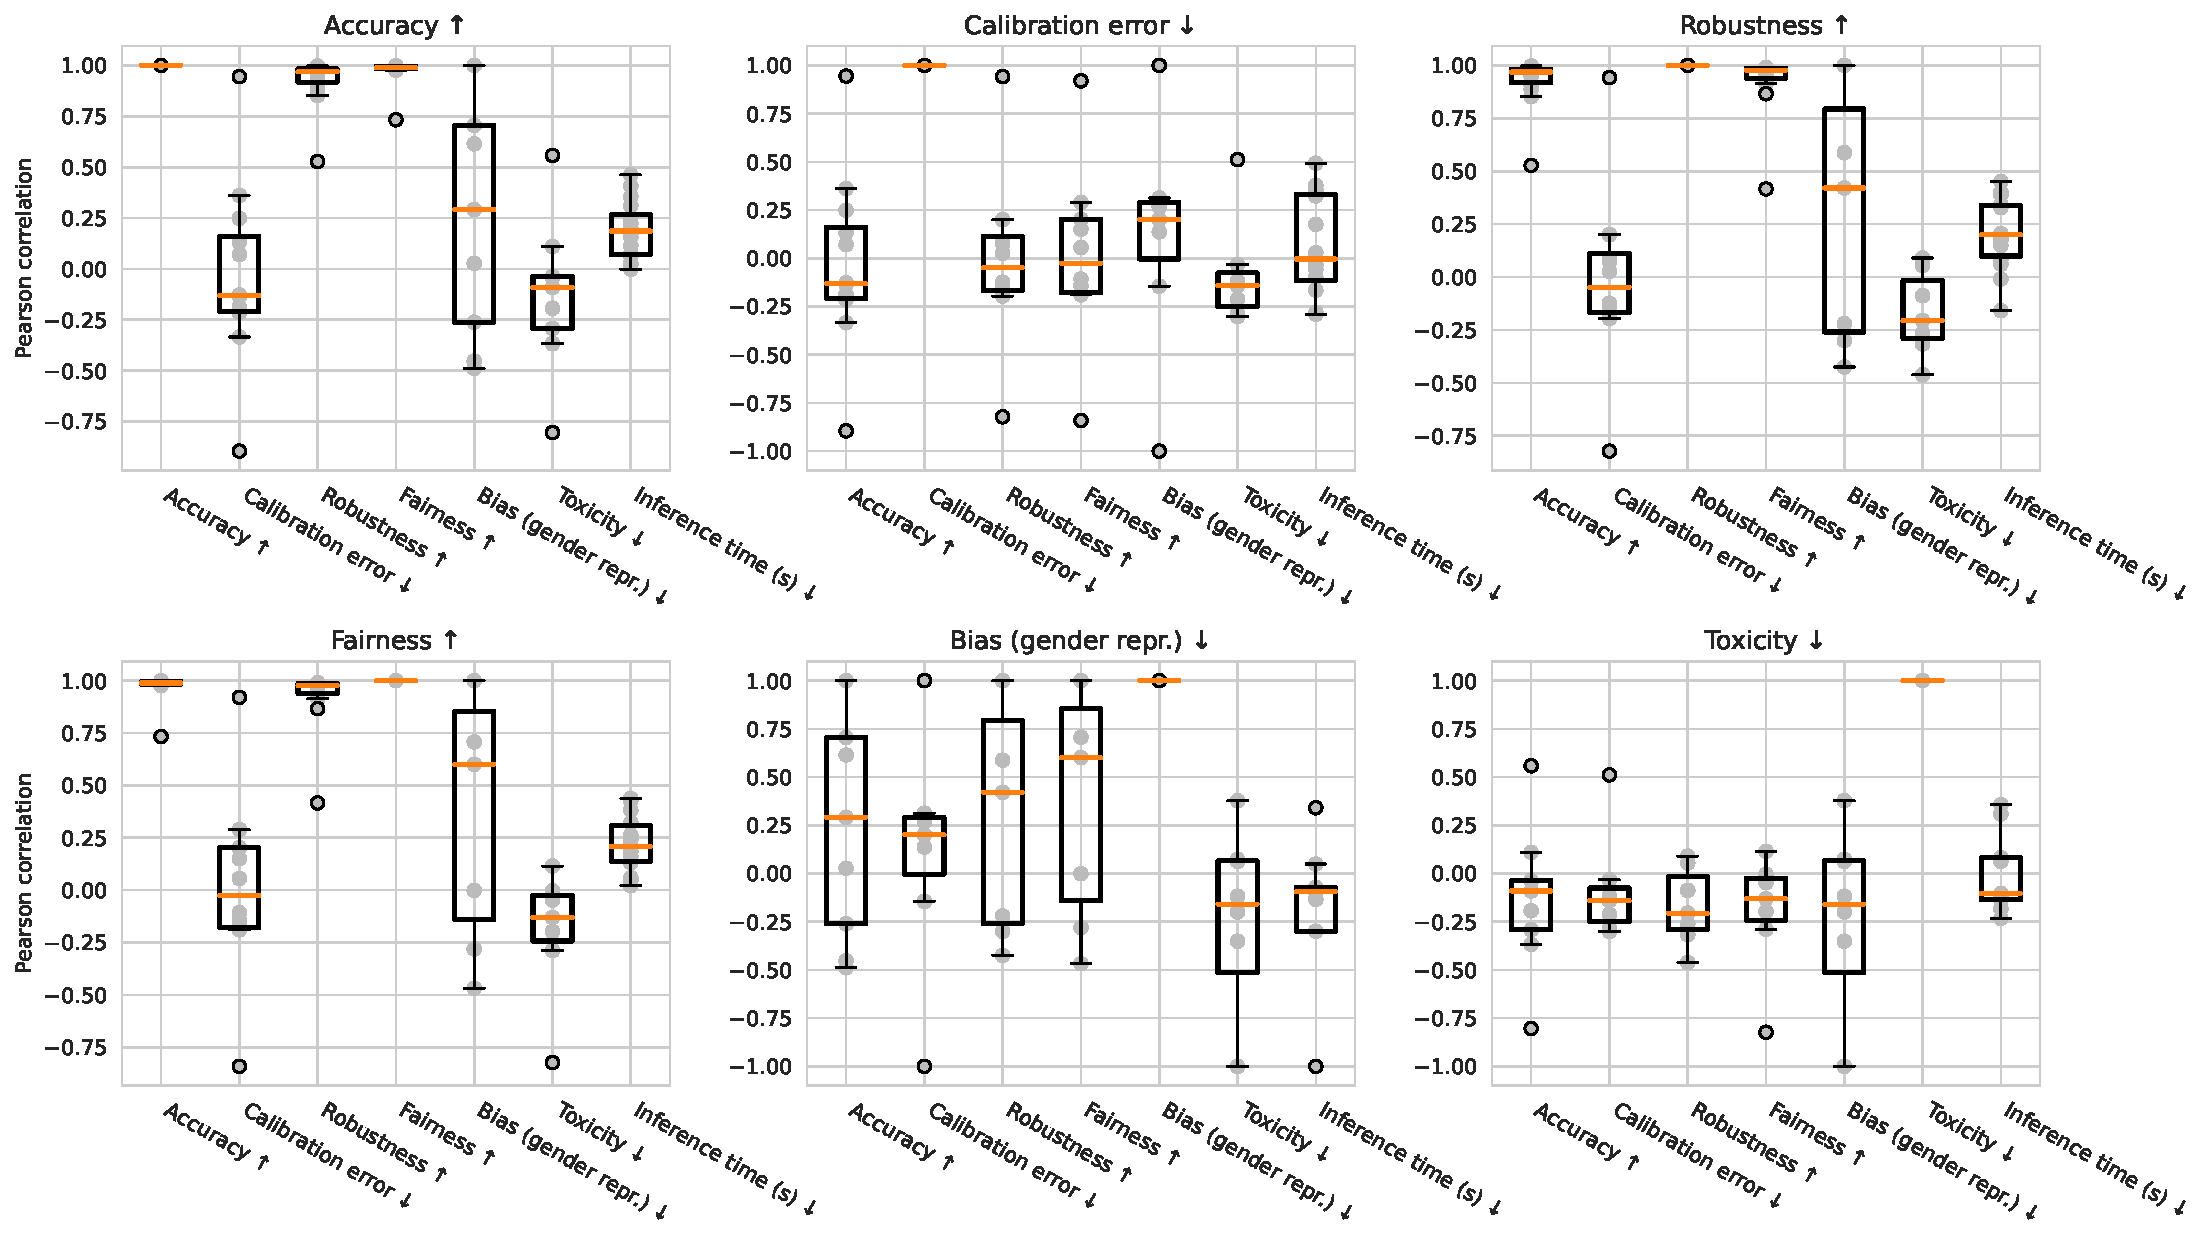
\includegraphics[width=\textwidth]{plots/metric_correlation.pdf}
  \caption{\textbf{Correlation between metrics.} The Pearson correlation between each metric and every other metric (x-axis).
  The small grey dots denote the correlation on each individual scenario.
  Trends are qualitatively similarly for other correlation measures (\eg Spearman correlation).
  For calibration error, we measure ECE-10; for bias, we measure bias in gender representation; and for efficiency, we measure denoised inference time. 
  }
  \label{fig:inter-metric-correlations}
\end{figure*}

\paragraph{Inter-metric relationships.}
A central tenet of our holistic evaluation is to foreground metrics beyond accuracy, ensuring that the many desiderata we should expect of systems are indeed measured for each scenario (when possible; see \reftab{scenarios-metrics-matrix}).
As a consequence, this clarifies how different metrics relate to each other.
Many prior works have explored these types of relationships extensively for specific metric pairs: for example, accuracy-robustness \citep{miller2021line, koh2021wilds}, accuracy-efficiency \citep{coleman2017dawnbench}, calibration-fairness \citep{pleiss2017, jones2021selective}, and bias-toxicity \citep{sap2019risk, halevy2021mitigating}.
In the context of language models, we may posit the relationships found in prior works will continue to bear, but many pairs have not been studied and we do not have definitive evidence that these relationships hold up reliably.

Therefore, we harness our evaluation's coverage of these metrics to provide two resources.
First, in \reffig{acc-X}, we depict the relationship between accuracy and each of the \numnonaccuracymetriccategories other desiderata.
Among other interpretations, this figure helps clarify when more accurate systems coincide with improvements in other key desiderata and when there are important trade-offs.
Further, by plotting these on a per-scenario basis, this helps to showcase the underlying heterogeneity in the trends: when are metric relationships consistent across scenarios, when are they highly scenario-dependent, and what are the anomalies?
Second, in \reffig{inter-metric-correlations}, we consolidate the relationship across models for specific scenarios.
Concretely, in each subfigure we consider a pair of metrics, where each grey point corresponds to the Pearson correlation (\ie linear fit) between these metrics across all models for this scenario.\footnote{We also considered Spearman correlation (\ie monotonic fit), given this may be more appropriate for some metric relationships, but found the qualitative trends to be largely invariant across these two choices of correlations metrics.}
Once again, this helps to showcase the spread and heterogeneity in pairwise metric relationships as well as the macro-level trends.

While these figures together provide a wealth of information, we step through them to state specific takeaways.
Most strikingly, we find that across all scenarios, accuracy, robustness, and fairness are extremely strong correlated (see \reffig{inter-metric-correlations}).
In part, we believe this is a finding contingent on how we chose to measure robustness/fairness.
For robustness, this aligns with findings for other forms of (non-adversarial) robustness, such as the work of \citet{miller2021line} for distributional robustness, which shows in-domain and out-of-domain accuracy lie on a line.
On the other hand, for fairness, we find this to be quite surprising.
We do emphasize several prior works instead find trade-offs between fairness and accuracy, but we do not believe that our work should be interpreted as contradicting their findings.
Not only do we measure fairness differently from these works, but the setting of few-shot prompting of language models is considerably different from the settings studied in these prior works \citep{zhang2019theoretically, raghunathan2020understanding, dutta2020tradeoff, wang2021understanding, zhao2022inherent}. 

Shifting focus to calibration, the trends are more scenario-dependent, as can be seen for accuracy by the visual clustering of points for a given scenario in \reffig{acc-X}. 
Strikingly, we find that the relationship between accuracy and calibration can be quite different for very similar scenarios: for two commonsense-centric QA scenarios, we see accuracy and calibration are highly correlated in \openbookqa (correlation of greater than 0.8) whereas accuracy and calibration \textbf{error} are highly correlated in \hellaswag (correlation greater than 0.85). 
Further, while not unsurprising given the strong correlations between accuracy, robustness, and fairness, the finding that more robust and more fair models can be less well-calibrated is counter-intuitive and surprising.

For generative harms, we also see significant variation in the relationship with other metrics.
For toxicity, the correlations on average with other metrics are near zero as the toxicity rates themselves for toxicity are relatively constant and near zero, with the clear exception of \narrativeqa in \reffig{acc-X}. 
In contrast for bias, we see some positive correlation between accuracy and gender representation bias (lower is better), with an even more striking average correlation of scenarios of more the 0.5 between fairness (higher is better) and gender representation bias (lower is better). 
In other words, we see a clear and surprising trade-off: models that tend to have better fairness performance, which depends on task-specific performance, tend to have worse gender bias, which depends on model generations but not task-specific performance.
As to the two generative harms, we see there are some scenarios where they are fairly anti-correlated, which indicates the less gender biased models tend to be more toxic for these scenarios.
These findings indicate it may not suffice to only measure one of these types of harms, and that efforts to reduce one may have side-effects for the other \citep[\cf][]{xu2021detoxifying}, which is especially relevant given the harms of toxicity are more straightforward/immediate (\eg more likely to draw media/journalistic attention) whereas the harms of bias may be more subtle/gradual. 

Finally, for efficiency, we see fairly weak correlations with other metrics.
In particular, we do not see a strong overarching trade-off between accuracy and efficiency, which we may have anticipated \textit{a priori}.
This is made clear by \reffig{acc-X}, which instead showcases that the trends for efficiency tend to be quite scenario-dependent.
This is especially true for the denoised metric, given a lot of what drives the measurements relates to the fundamental distributional properties of the scenario (\ie the length of inputs and outputs).

\paragraph{Direct model comparisons.}
A central objective for our evaluation is to achieve common and unified understanding of all the models available.
In particular, as we document in \refapp{benchmark-comparison}, the \nummodels models we evaluate in this work have been previously evaluated under different conditions for different evaluation suites.
In particular, the degree of overlap is surprisingly low and uneven across different models.
Consequently, we lack clarity as a field on the relationship between different models.

\begin{figure}
\centering
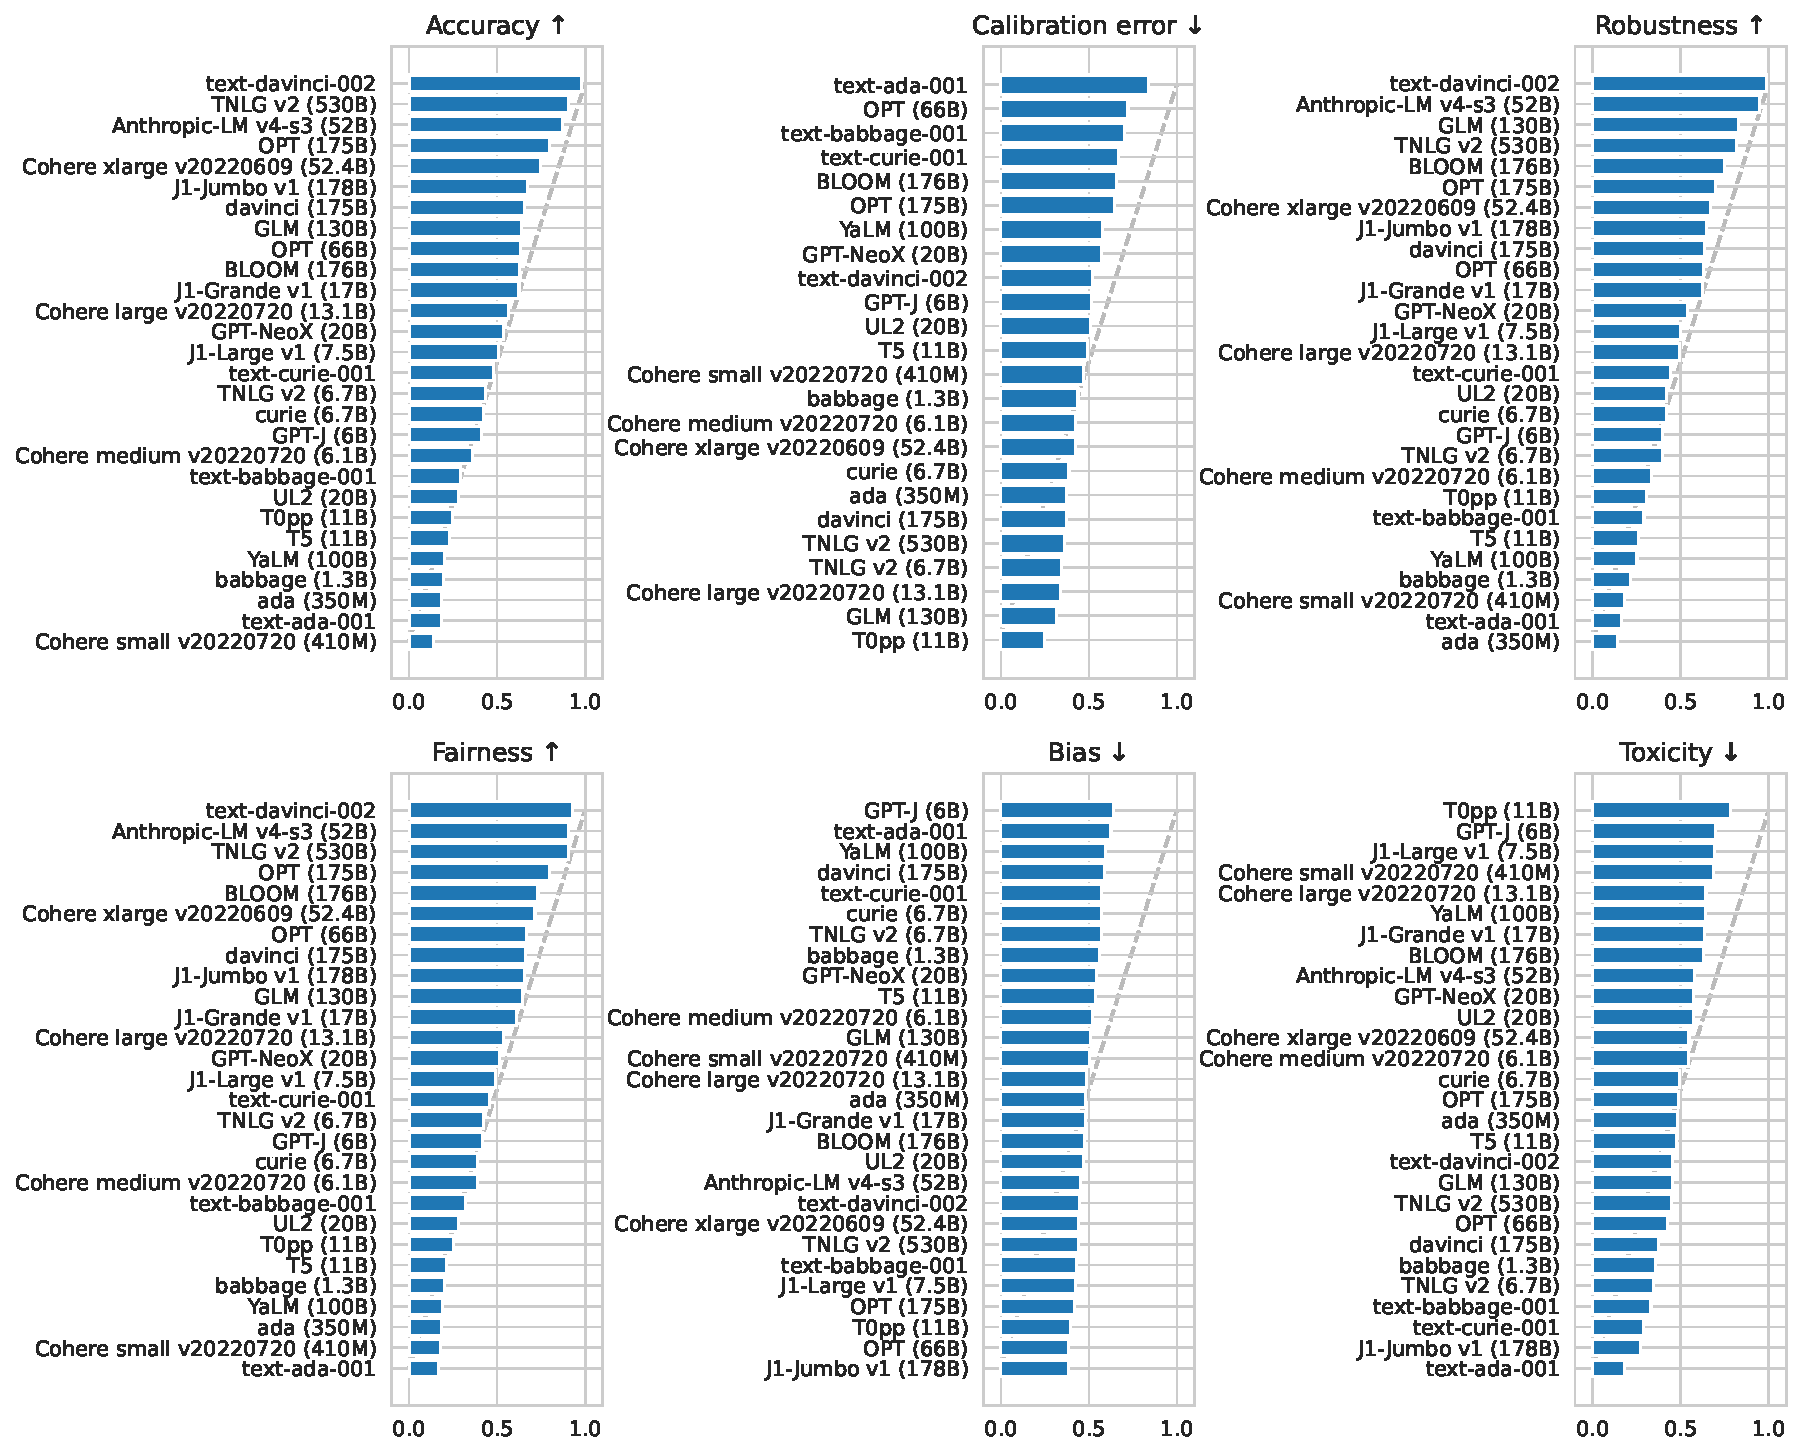
\includegraphics[width=\textwidth]{plots/model_ranking_all.pdf}
  \caption{\textbf{Head-to-head win rate per each model.} 
  We report the fraction of head-to-head comparisons between the given model and all other models, across all scenarios, where the given model is higher along the metric (\eg more accurate in the accuracy subfigure).
  If a model was the highest for the given metric for every scenario, it would receive a score of 1.0; if a model received a score of 0.5, then if a scenario and second model were chosen at random, the outcome of the comparison would be a coin flip.
  For metrics where higher is better (Accuracy, Robustness, Fairness), the better models are towards the top, and vice versa.
  For calibration error, we measure ECE-10; for bias, we measure bias in gender representation; and for efficiency, we believe these comparisons should not be made without consideration of accuracy and they are further discussed in \citet{narayanan2022evaluating}. 
  }
  \label{fig:head-to-head}
\end{figure}

In \reffig{head-to-head}, we report how different models would fare in a head-to-head comparison for each metric across all the \core scenarios.\footnote{We exclude efficiency as we believe head-to-head comparisons based solely on efficiency are not meaningful; instead efficiency needs to be considered in conjunction with other metrics like accuracy. Forthcoming work~\citep{narayanan2022evaluating} examines the tradeoffs between accuracy and efficiency.
}
We find that \instructdavinci is clearly the most accurate model, winning in these comparisons more than 90\% of the time.
Of the remaining models, we see that the largest model \mtnlgfivethreezero is the second most accurate, followed by \anthropic.
In light of the significant difference in model scale of a factor of more than 10 between \mtnlgfivethreezero and \anthropic, given \instructdavinci and \anthropic share instruction-tuning in common (which other models, beyond smaller OpenAI text variants, do not), this suggests that instruction-tuning and the use of human feedback is an efficient and effective  means for improving model accuracy.

Further, while we will later see the overall relationship between model scale and accuracy can be complicated (\reffig{scale-accuracy}), here we see a clear thresholding effect in terms of model scale.
All of the models with a win rate for accuracy clearly above chance (\eg 55\% or more) have more than 50B parameters, whereas the sole exception of a large model outside this group of the top 10 is \yalm.
\yalm has a surprisingly poor accuracy win rate below 25\%, perhaps because of significant training on Russian instead of English). 
Within the top 10, we see model scale appears to be less predictive of rank, as two of the largest models (\bloom and \jurassicjumbo; both 100B+ parameters) are at the bottom of this tier, whereas \anthropic and \coherexl (the two smallest models in the tier) are in the top half of this tier.
Similarly, within a model family, we see model scale is perfectly monotonically correlated with model accuracy win rate (\eg see the OpenAI and Cohere model variants). 
We emphasize this certainly does not imply the models that fare poorly, or the small models, are inaccurate under all conditions: we expect that the prompting approaches we used are poorly suited for these smaller models and, perhaps, it is better to fine-tune these models \citep[\cf][]{liu2022fewshot}.

Consistent with previous findings of accuracy being correlated with robustness and fairness, we see similar rankings of models for those scenarios.
However, we note that \bloom notably performs considerably better (in a relative sense) for robustness/fairness than its accuracy would suggest, with \optonesevenfive and \glm roughly interchanging positions for robustness and accuracy (\ie \glm is more robust and less accurate in a relative sense compared to \optonesevenfive). 
In contrast, perhaps also as expected given the weak correlations of generative harms with other metrics, we see the rankings for toxicity and bias are notably quite different.
We highlight how \tzero and \gptdavinci in particular demonstrate the opposite trends when comparing their bias win rates to their toxicity win rates.
That is, \tzero is the most toxic when compared to all other models, but one of the three least (gender) biases, whereas \gptdavinci is one of the four most biased head-to-head, but one of the less toxic models.  

\begin{figure}
\centering
  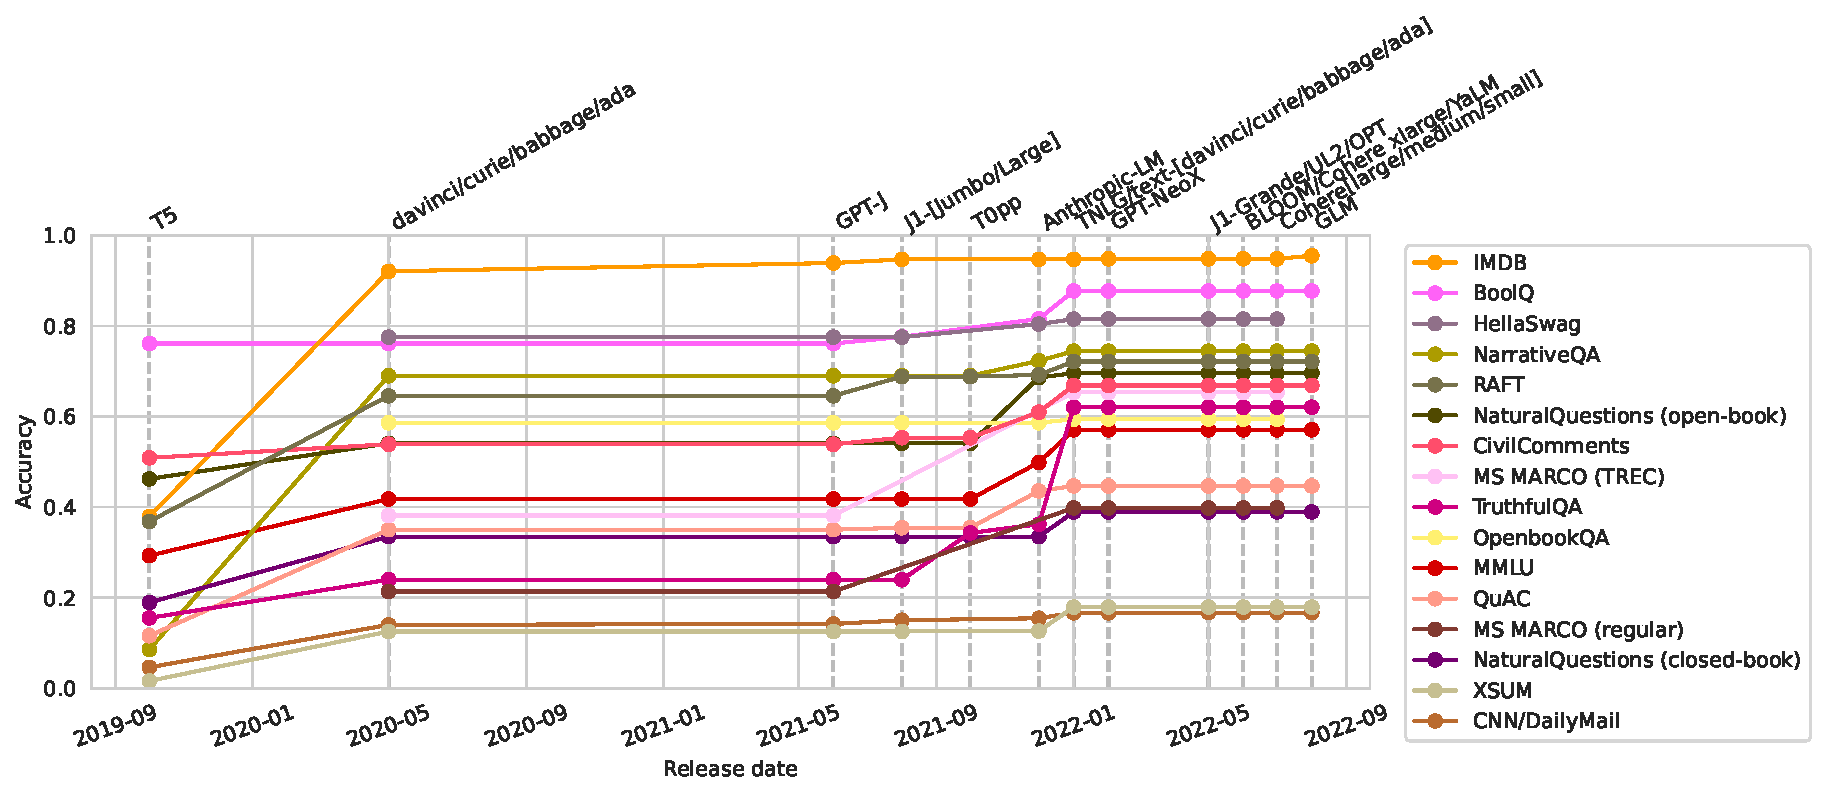
\includegraphics[width=\textwidth]{plots/accuracy_over_time.pdf}
  \caption{\textbf{Cumulative accuracy over time.} The relationship between time (x-axis) and the accuracy of the most accurate model released up to that point (y-axis) across \numcorescenarios \core scenarios. 
  That is, the graph tracks the progress in the state-of-the-art (SOTA) accuracy over time for each scenario.
%   \todo{Dimitris: fix overlaps}
  }
  \label{fig:accuracy-over-time}
\end{figure}

\begin{figure}
\centering
  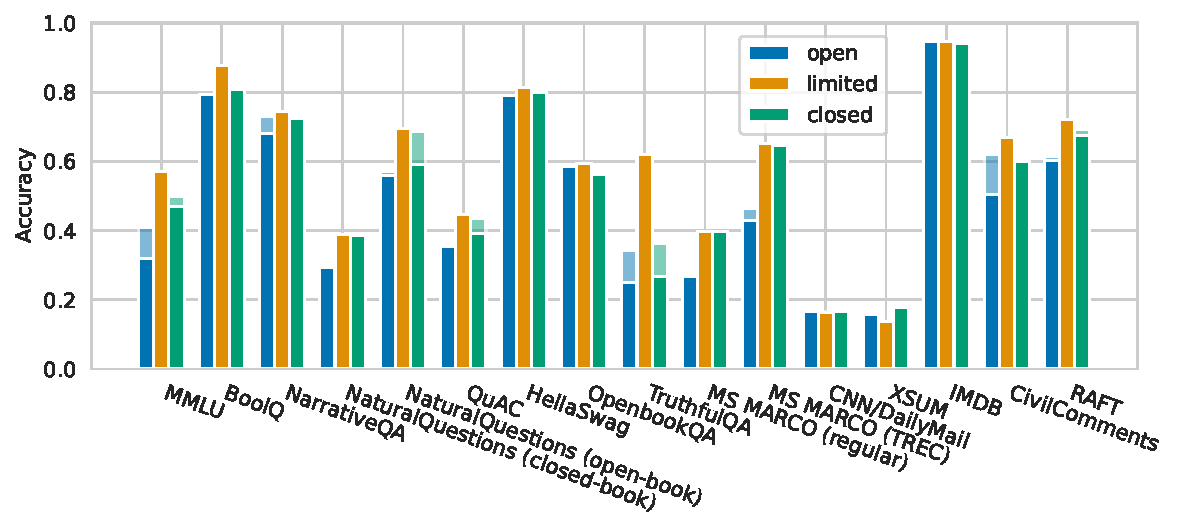
\includegraphics[width=0.85\textwidth]{plots/accuracy_v_access.pdf}
  \caption{\textbf{Accuracy as a function of model access.} The relationship between access (\textbf{open} vs. \textbf{limited} vs. \textbf{closed}) and model accuracy for each of the \numcorescenarios \core scenarios. Shaded bars indicate the performance of the best model for that scenario, whereas the solid bars indicate the performance of the overall most accurate model across all \core scenarios based on \reffig{head-to-head}.} 
  \label{fig:accuracy-vs-access}
\end{figure}

\paragraph{Accuracy as a function of other variables.}
To build on these model comparisons, we now consider trends in model accuracies as a function of other relevant variables. 
In \reffig{accuracy-over-time}, we report model accuracies as a function of time (\ie model release date). 
As a function of time, we see that the release of GPT-3 \citep{brown2020gpt3} clearly establishes a strong baseline for future models across all scenarios, with a distinctive improvement over \tfive.
To the extent there is upward movement in accuracy since then, we often see it coming with the introduction of \anthropic roughly 18 months later in December, 2021 (the first model to use reinforcement learning with human feedback of those we evaluate), though we see a surprisingly clear monotonic improvement over the intermediary period for \naturalquestions. 

In \reffig{accuracy-vs-access}, we stratify the results for accuracy based on model accessibility \citep[see][]{liang2022community-norms} as we discuss in \refsec{models}.
For each access category, we report the per-scenario accuracy of the model in that category that is the most accurate (full bar) and that is generally the most accurate (smaller dark sub-bar; based on \reffig{head-to-head}).
This means the sub-bar is always the accuracy of \optonesevenfive for \textbf{open} models, \instructdavinci for \textbf{limited access} models, and \mtnlgfivethreezero for \textbf{closed} models.
We see that these models for \textbf{limited} access are consistently the best in their categories, but \optonesevenfive is sometimes improved over (\eg 10 point improvement for \mmlu and \civilcomments) as is \mtnlgfivethreezero (\eg more than 5 point improvement for \naturalquestions (open-book) and \truthfulqa).

Overall, we see the accuracies generally fall in the direction \textbf{limited access} > \textbf{closed} > \textbf{open}, which aligns with \reffig{head-to-head}. 
With that said, we see some reason for optimism regarding open science through open-sourced models, in that the best public model is usually somewhat competitive in accuracy (\ie within 5 points of the best non-open model), with the notable exceptions of more knowledge-intensive scenarios of \mmlu, \naturalquestions (closed-book) and \truthfulqa as well as both information retrieval scenarios. 
This is especially noteworthy given we have yet to see models being open-sourced with significant use of human preferences and reinforcement learning from human feedback, which may further bridge this gap.
However, we do highlight there are other confounds: some models may not be disclosed to the public (let alone released), some models may be disclosed after significant delay, and some highly accurate models are not yet evaluated in \benchmarkname (\eg Gopher, Chinchilla, PaLM; see \refsec{missing-models}).
We hope our findings on the relationship between model accessiblity and model performance (\eg accuracy) will inform the development of community norms and standards around model access/release \citep{liang2022community-norms}. 

\begin{figure}
\centering
  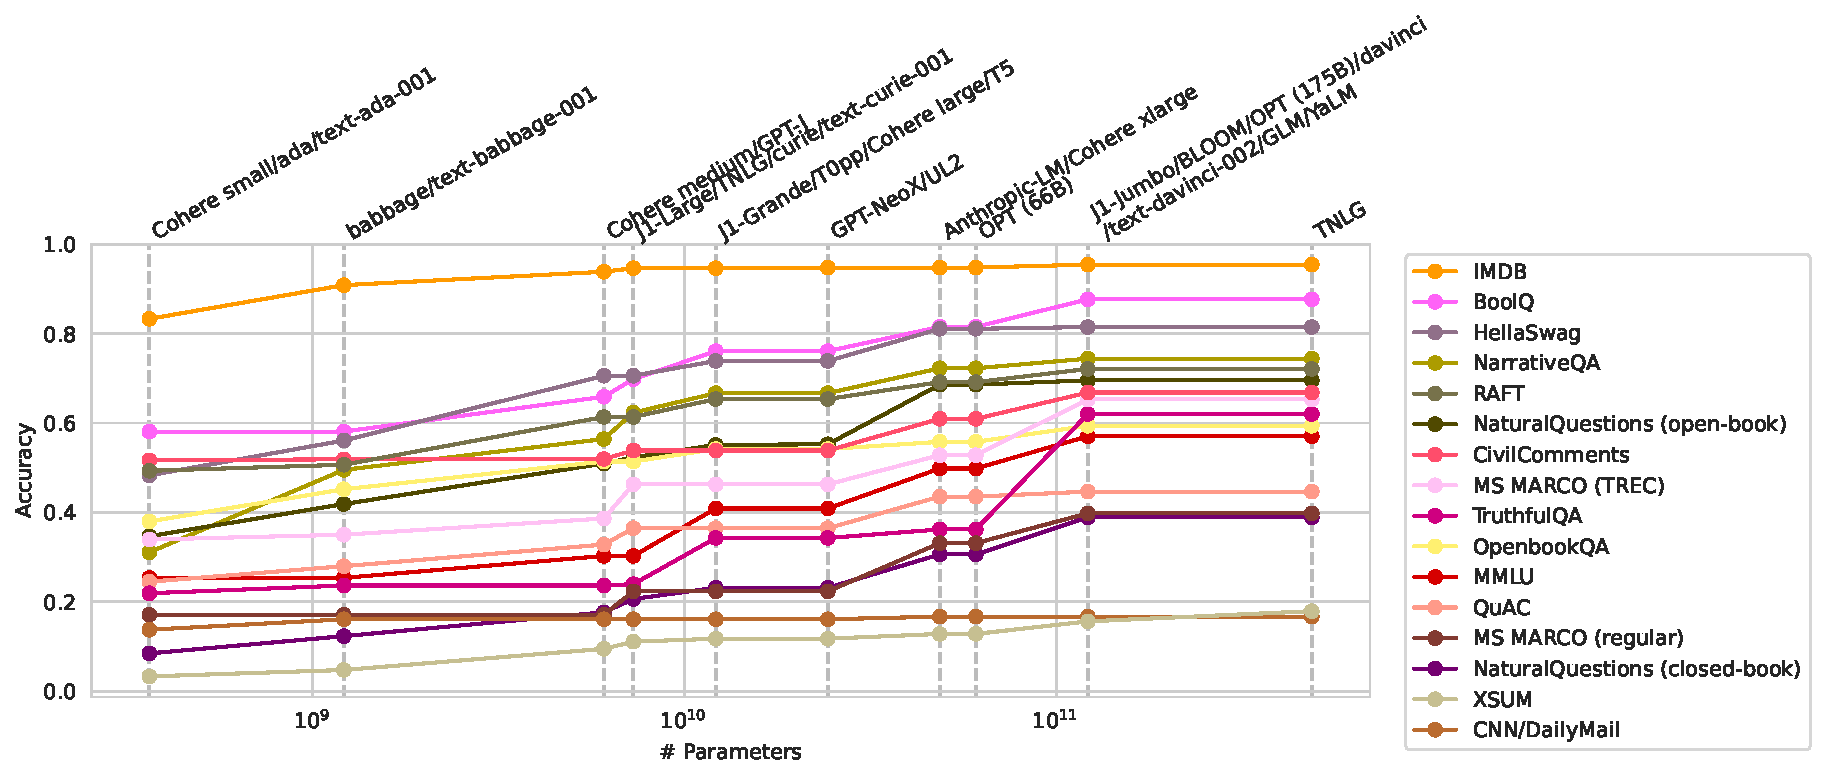
\includegraphics[width=\textwidth]{plots/accuracy_v_parameters.pdf}
  \caption{\textbf{Cumultative Scale vs. Accuracy.} 
    The relationship between model parameter size (x-axis) and the accuracy of the most accurate model released up to that scale on each \core scenario.
    That is, the graph tracks the progress in the state-of-the-art (SOTA) accuracy as a function of scale for each scenario.
  }
  \label{fig:scale-accuracy}
\end{figure}

\begin{figure}
\centering
  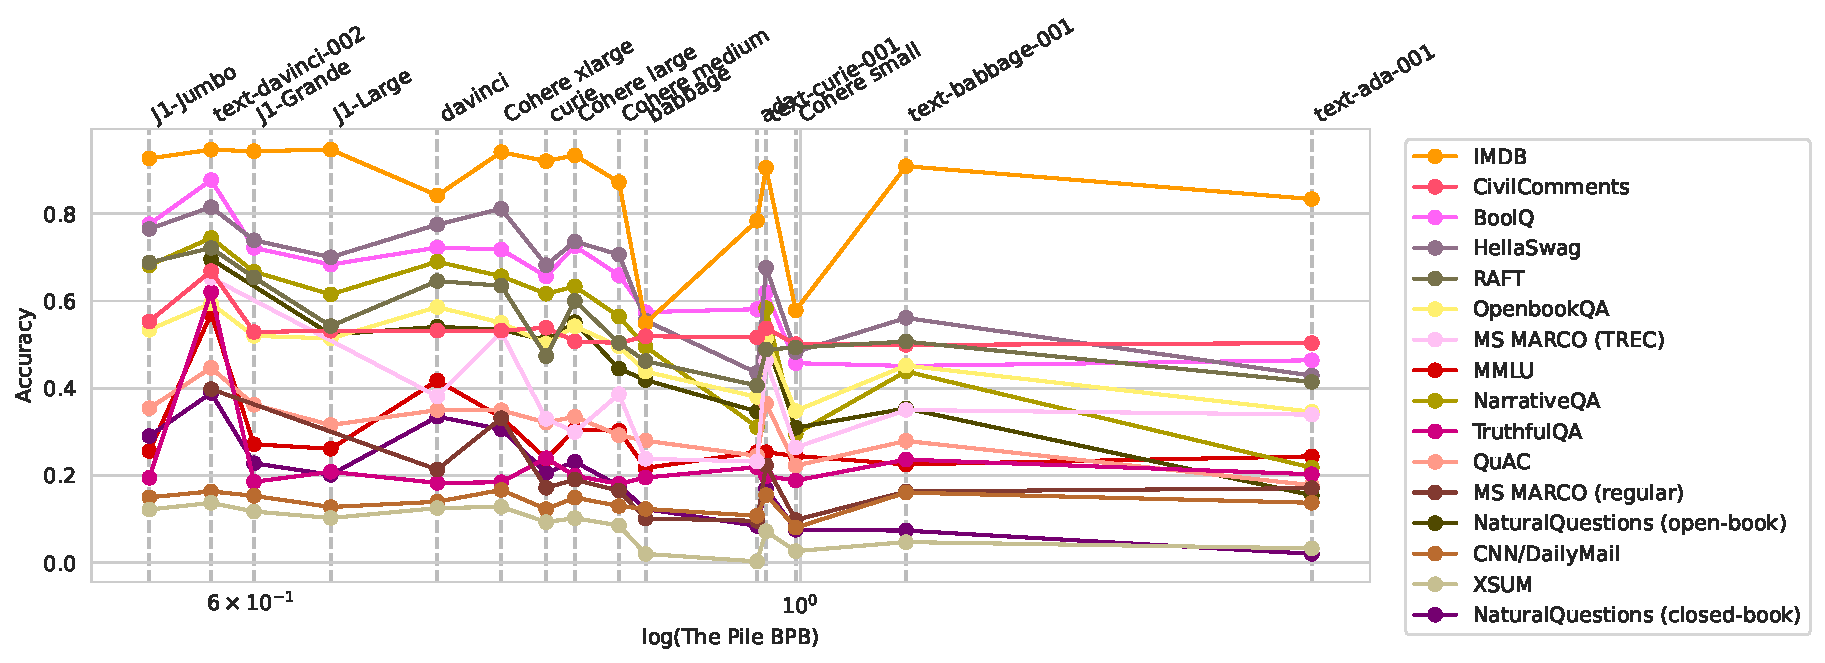
\includegraphics[width=\textwidth]{plots/accuracy_v_bpb.pdf}
  \caption{\textbf{\pile loss vs. Accuracy.} The relationship between log bits-per-byte (BPB) on \pile and the accuracy on each \core scenario.}
  \label{fig:perplexity-accuracy}
\end{figure}

\paragraph{Predicting accuracy.}
Given the resource-intensive nature of producing language models, especially the most capable models (for which we take accuracy for different scenarios as a proxy), the ability to predict model capabilities\footnote{It would be similarly interesting to predict our properties (\eg those related to harms), though here we focus on accuracy. We do note that our evaluation deliberately surfaces all the necessary metrics required to project other properties.} is valuable for orienting decision-making.
Prior work demonstrates model scale (whether measured in model size, data size, or compute/training FLOPs) reliably predicts model loss for language models, establishing \textit{scaling laws} \citep{kaplan2020scaling, hoffmann2022chinchilla}.
On the other hand, work has also shown that certain qualitative capabilities \citep[\eg in-context learning;][]{brown2020gpt3} \textit{emerges} unpredictably beyond a critical scale threshold \citep[see][]{wei2022emergent}.
And many works have implicitly assumed and demonstrated that improvements in language modeling loss (\ie perplexity) translate to improvements on downstream use cases. 
In \reffig{scale-accuracy}, we report on the relationship between model scale and accuracy, while in \reffig{perplexity-accuracy}, we report perplexity (measured on \pile) vs. accuracy.

In light of the very consistent picture that model scale within a family led to reliable improvements in accuracy (\reffig{head-to-head}), we see that this does not generalize across model families.
If we are to plot model scale vs. accuracy, we find the relationship is very chaotic; model scale (agnostic to model family) as measured in parameters is a poor predictor of trends in accuracy.
Unfortunately, the data on different models was too sparse to attempt a similar analysis in terms of training FLOPs, but we expect such an analysis may be more helpful in demonstrating a crisper relationship between training compute and downstream accuracy.
When we accumulate the performance of models in \reffig{scale-accuracy}, so as to understand if scale appears more necessary to improve accuracy, we do see some notable jumps for many scenarios both in the range of 12B parameters and 50B parameters.
These jumps are specifically attributable to \tzero and \anthropic, which likely instead indicates that attributing these jumps to scale is confounded by other changes (\ie the training procedure of \tzero to deliberately improve few-shot prompting performance and the RLHF involved in \anthropic).
And we similarly see the relationship between perplexity (or, more accurately, log bits-per-byte) on \pile and downstream accuracy is similarly messy (\reffig{perplexity-accuracy}), though we expect the confound of contamination (some models are trained on \pile and others are not) exacerbates the messiness of these findings.